%%%%%%%%%%%%%%%%%%%%%%%%%%%%%%%%%%%%%%%%%%%%%%%%%%%%%%%%%%%%%%%%%%%%%%%%
%    INSTITUTE OF PHYSICS PUBLISHING                                   %
%                                                                      %
%   `Preparing an article for publication in an Institute of Physics   %
%    Publishing journal using LaTeX'                                   %
%                                                                      %
%    LaTeX source code `ioplau2e.tex' used to generate `author         %
%    guidelines', the documentation explaining and demonstrating use   %
%    of the Institute of Physics Publishing LaTeX preprint files       %
%    `iopart.cls, iopart12.clo and iopart10.clo'.                      %
%                                                                      %
%    `ioplau2e.tex' itself uses LaTeX with `iopart.cls'                %
%                                                                      %
%%%%%%%%%%%%%%%%%%%%%%%%%%%%%%%%%%
%
%
% First we have a character check
%
% ! exclamation mark    " double quote  
% # hash                ` opening quote (grave)
% & ampersand           ' closing quote (acute)
% $ dollar              % percent       
% ( open parenthesis    ) close paren.  
% - hyphen              = equals sign
% | vertical bar        ~ tilde         
% @ at sign             _ underscore
% { open curly brace    } close curly   
% [ open square         ] close square bracket
% + plus sign           ; semi-colon    
% * asterisk            : colon
% < open angle bracket  > close angle   
% , comma               . full stop
% ? question mark       / forward slash 
% \ backslash           ^ circumflex
%
% ABCDEFGHIJKLMNOPQRSTUVWXYZ 
% abcdefghijklmnopqrstuvwxyz 
% 1234567890
%
%%%%%%%%%%%%%%%%%%%%%%%%%%%%%%%%%%%%%%%%%%%%%%%%%%%%%%%%%%%%%%%%%%%
%
\documentclass[12pt]{iopart}
%\newcommand{\gguide}{{\it Preparing graphics for IOP journals}}
%Uncomment next line if AMS fonts required
%\usepackage{iopams}
\usepackage{graphicx}

\begin{document}

\title{Iconic representations of molluscs through the ages}

\author{Mattias T Johnsson$^1$, Graham R Dennis$^2$ and Joseph J Hope$^1$}

\address{$^1$Department of Quantum Science, Research School of Physics and Engineering, The Australian National University, Canberra ACT 0200, Australia}
\address{$^2$Plasma Research Laboratory, Research School of Physics and Engineering, The Australian National University, Canberra ACT 0200, Australia}
\ead{mattias.johnsson@anu.edu.au}

\begin{abstract}
More squeezing than you can shake a stick at.

\end{abstract}

%Uncomment for PACS numbers title message
%\pacs{00.00, 20.00, 42.10}
% Keywords required only for MST, PB, PMB, PM, JOA, JOB? 
%\vspace{2pc}
%\noindent{\it Keywords}: Article preparation, IOP journals
% Uncomment for Submitted to journal title message
%\submitto{\JPA}
% Comment out if separate title page not required
\maketitle

\section{Introduction}
\label{sectionIntroduction}
\begin{itemize}
  \item General non-classical state generation with atoms
  \item Talk about number squeezing with atoms
  \item Link to interferometry
  \item Motivate why large number squeezing
  \item Point out no one has done it before, only low number squeeze
  \item Lay out what sections we have and what we've done
\end{itemize}

\section{Model and two mode solutions}
\label{secTwoModeAnalytic}
\begin{itemize}
  \item Lay out the scheme with diagram, define all variable etc
  \item Present multimode analytic solution, details go into an appendix
  \item Plot a few solutions to give an idea of what things look like, plausible times and so on
  \item Maybe point out it agrees with Oberthaler, or save that for discussion on MM effects?
  \item Point out that number *difference* squeezing can often be considerably higher than absolute number squeezing in a single state
\end{itemize}

As our goal is to describe the number squeezing possibilities of a two component BEC, we begin by considering a simplified version of the problem, consisting of a two-mode system, with the modes corresponding to the two states of the condensate. In the full problem, each of the components will include many spacial modes; our two mode system makes the assumption that only one of these spacial modes is relevant for each of the condensate's components.

{\bf{Maybe expand on the link between a full BEC in a trap and a the following hamiltonian?}}

We allow the atoms to interact via a standard Kerr-type nonlinearity arising from atom-atom interactions, as well as allowing a linear coupling between the two modes. Denoting the two modes by $|a\rangle$ and $|b\rangle$, the Hamiltonian governing this system is given by
\begin{equation}
\hat{H} = \hbar \omega \hat{a}^{\dagger} \hat{a} +  \hbar \omega \hat{b}^{\dagger} \hat{b} 
          + \frac{\chi_{aa}}{2} \hat{a}^{\dagger} \hat{a}^{\dagger} \hat{a} \hat{a}
          + \chi_{ab} \hat{a}^{\dagger} \hat{a} \hat{b}^{\dagger} \hat{b}
          + \frac{\chi_{bb}}{2} \hat{b}^{\dagger} \hat{b}^{\dagger} \hat{b} \hat{b}
          + \Omega (\hat{a}^{\dagger} \hat{b} + \hat{b}^{\dagger}  \hat{a} )
\label{eqTwoModeHamiltonian}
\end{equation}
where the $\chi_{ij}$ describe the various inter- and intra-mode nonlinearities, and $\Omega$ couples the two modes and allows for population transfer between them.

The system is prepared with all the population in $|a\rangle$, and vacuum in $|b\rangle$. $|a\rangle$ is well-described by a coherent state {\bf *** Justify this. ***} with average number $\langle \hat{a}^{\dagger} \hat{a} \rangle = N$, where $N$ is the total particle number in our system.

At time $t=0$ the coupling $\Omega$ is switched on and applied until time $t=t_1$, at which point it is turned off, resulting in a portion of the population being transferred into mode $|a\rangle$. As the initial state was a coherent state in both modes, after the population transfer both $|a\rangle$ and $|b\rangle$ are described by coherent states, with mean number $\langle \hat{a}^{\dagger} \hat{a} \rangle = n_a$ and $\langle \hat{b}^{\dagger} \hat{b} \rangle = n_b$ respectively.

The coupling $\Omega$ is then switched off until time $t_2$. During this period the atoms interact solely through the nonlinear terms, with no population being transferred. Due to the form of the Hamiltonian, the number variance remains unchanged, but the quadrature variances in the two modes change over time, which can lead to quadrature squeezing \cite{xxx}.

After this hold time $\tau_{\mathrm{hold}} = t_2 - t_1 $, the coupling $\Omega$ is switched back on until time $t_3$, with a phase shift $\phi$ compared to it's first application. During this last stage, the two modes exchange population and the quadrature variance is converted into number variance, in the same way homodyne measurements are used in quantum optics to convert quadrature squeezing (which cannot be directly measured) into number squeezing (which can). In this interpretation, $\phi$ is the relative phase of the strong local oscillator, which allows specific phase angles of quadrature squeezing to be examined.

In another interpretation, the sequence of pulses results in a Ramsey interferometer, with a final beam splitter phase of $\phi$.

The entire sequence of pulses and the resulting populations are shown schematically in Figure~\ref{figPulseScheme}.

This system can be solved analytically, and expressions for quadrature, absolute and relative number squeezing can be derived. We present the solutions here; the full derivation can be found in \ref{appendixTwoModeDerivation}.
If we define
\begin{eqnarray}
s &=& \sin(\Omega (t_3 - t_2)) \\
c &=& \cos(\Omega (t_3 - t_2)) \\
\lambda_{ij} &=& \chi_{ij} \tau_{\mathrm{hold}} / \hbar \\
A &=& \sqrt{n_a} \exp [n_a (e^{-i(\lambda_{aa}-\lambda_{ab})} - 1 )] \\
A_2 &=& n_a \exp [n_a (e^{-2i(\lambda_{aa}-\lambda_{ab})} - 1 )] \\
B &=& -i e^{i \phi}\sqrt{n_b} \exp [n_b (e^{-i(\lambda_{bb}-\lambda_{ab})} - 1 )] \\
B_2 &=& -n_b e^{2i\phi} \exp [n_b (e^{-2i(\lambda_{bb}-\lambda_{ab})} - 1 )] \\
D &=& AB^* - A^*B
\end{eqnarray}
then the expectation values for number, number variance, and number difference variance after appling the final coupling field for a time $\tau = t_3-t_2$ are given by
\begin{eqnarray}
N_a(t_3) &=& n_a c^2 + n_b s^2 + i c s D \\
%
N_b(t_3) &=& n_a s^2 + n_b c^2 - i c s D \\
%
{\mathrm{Var}} [ N_a](t_3) &=& n_a c^2 + n_b s^2 + 2 n_a n_b c^2 s^2 \\
       && + c^2 s^2 (D^2 - e^{i(\lambda_{aa} - \lambda_{bb})} B_2 A_2^* - e^{-i(\lambda_{aa} - \lambda_{bb})} B_2^* A_2) \nonumber \\
       && + i c s D (1-2 n_a c^2 -2 n_b s^2)  \nonumber\\
       && + 2 i c^3 s n_a (e^{-i(\lambda_{aa} - \lambda_{ab})} A B^* - e^{i(\lambda_{aa} - \lambda_{ab})} A^* B ) \nonumber \\
       && + 2 i c s^3 n_b (e^{i(\lambda_{bb} - \lambda_{ab})} A B^* - e^{-i(\lambda_{bb} - \lambda_{ab})} A^* B ) \nonumber\\
%
{\mathrm{Var}} [ N_b](t_3) &=&  n_a s^2 + n_b c^2 + 2 n_a n_b c^2 s^2 \nonumber \\
       && + c^2 s^2 (D^2 - e^{i(\lambda_{aa} - \lambda_{bb})} B_2 A_2^* - e^{-i(\lambda_{aa} - \lambda_{bb})} B_2^* A_2 ) \nonumber \\
       && + i c s D (-1+2 n_a s^2 + 2 n_b c^2)  \nonumber \\
       && + 2 i c^3 s n_b (e^{-i(\lambda_{bb} - \lambda_{ab})} A^* B - e^{i(\lambda_{bb} - \lambda_{ab})} A B^* ) \nonumber \\
       && + 2 i c s^3 n_a (e^{i(\lambda_{aa} - \lambda_{ab})} A^* B - e^{-i(\lambda_{aa} - \lambda_{ab})} A B^* ) \\
%
{\mathrm{Var}} [ N_a - N_b](t_3) &=& n_a + n_b + 4 i c s D (n_a - n_b)(s^2 - c^2) \nonumber \\
       && + 4 c^2 s^2 (2 n_a n_b +D^2 - e^{i(\lambda_{aa} - \lambda_{bb})} A_2^* B_2 - e^{-i(\lambda_{aa} - \lambda_{bb})} A_2 B_2^* ) \nonumber \\
       && + 4 i c s (c^2 - s^2) (n_a e^{-i(\lambda_{aa} - \lambda_{ab})} A B^* - n_a e^{i(\lambda_{aa} - \lambda_{ab})} A^* B 
                     + n_b e^{-i(\lambda_{bb} - \lambda_{ab})} A^* B - n_b e^{i(\lambda_{bb} - \lambda_{ab})} A B^*)
\end{eqnarray}
In the case where all the nonlinearities are equal, such that $\chi_{aa} = \chi_{ab} = \chi_{bb}$, the number variances all reduce to those of a coherent state, e.g. ${\mathrm{Var}}[N_a]=N_a$, an no number squeezing is possible. 

There are three independent nonlinearities $\chi_{ij}$ in the Hamiltonian (\ref{eqTwoModeHamiltonian}). In the expressions for the number variances, however, the nonlinearities only appear in the cyclic combinations $\chi_{aa}-\chi_{ab}$, $\chi_{bb}-\chi_{ab}$ and $\chi_{aa}-\chi_{bb}$, meaning that number squeezing is parameterized by only two independent quantities which will be linear combinations of the nonlinearities. For example, since $\chi_{bb}-\chi_{ab} = (\chi_{aa}-\chi_{ab}) - (\chi_{aa}-\chi_{bb})$ it is possible to parameterize the number squeezing entirely in terms of the nonlinear differences $\chi_{aa}-\chi_{ab}$ and $\chi_{aa}-\chi_{bb}$.

{\bf{There seems to be this bogus rule of thumb in the literature that the amount of squeezing you can get is related to $\chi_{11}+\chi_{22}-2\chi_{12}$. Is it worth pointing out that this is wrong?}}

While the analytic expressions for the number variances are not particularly transparent, it is easy to evaluate and plot them for any given set of parameters. As an example, in Figure \ref{figxxx} we plot the solution for the normalized number variance in mode $|a\rangle$ for a particular set of nonlinearities, choosing a number of different values of $\phi$. The plots illustrate the basic features of the problem: During the final coupling period, the number variance undergoes cyclic variation, with a series of minima. It is necessary to choose both the correct phase $\phi$ as well as the correct length of time for the coupling to be applied in order to obtain optimum squeezing.




%Can Uaa + Ubb - 2Uab be zero and still get squeezing? Yep, Uaa=0.03, Ubb=0.01, Uab=0.2 gives squeezing for all quantities of interest



\begin{figure}
    \centering
    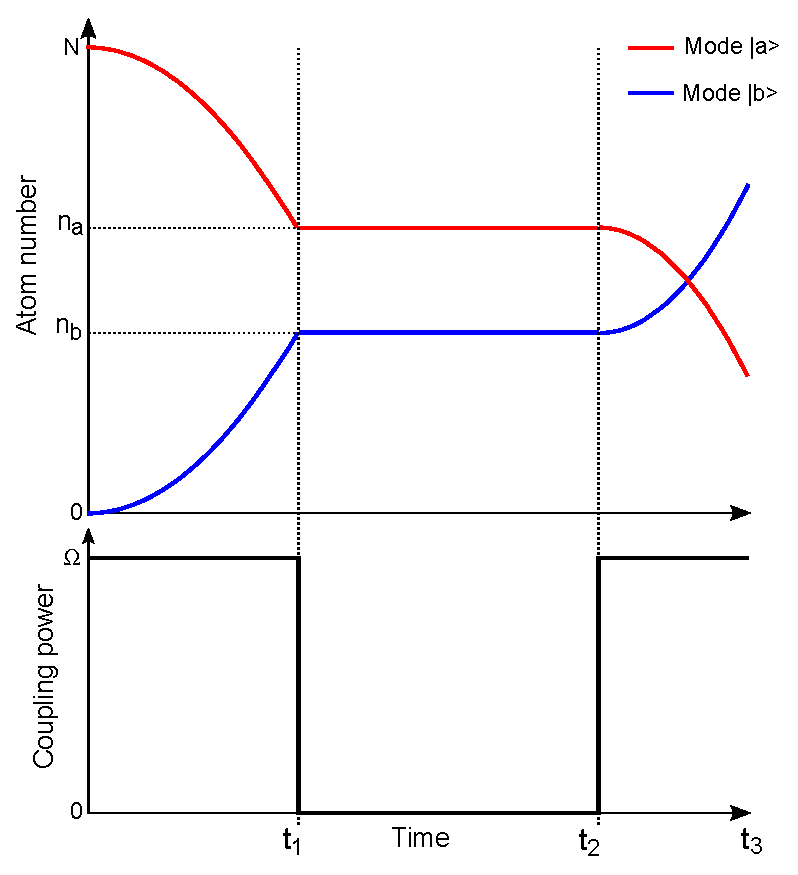
\includegraphics[width=8cm]{figures/pulse_scheme.eps}
    \caption{Mollusc mollusc}
    \label{figPulseScheme}
\end{figure}


\section{Multimode background section}
\begin{itemize}
  \item Motivate why MM analysis is necessary
  \item Brief recap why MM QFT is hard
  \item Say how great phase space methods are, quick overview of how they work, say only wigner works here, can probably crib some explanation and formulae from our fully quantum multimode atom laser paper
  \item Talk about all the checks I've done to make sure Wigner holds over the parameters we've simulated despite the fact that TWA is an uncontrolled approximation
  \item Cite XMDS, and say we're amazing at doing QFT sims, send money
  Derive link between mode shape, nonlinearity U, and the SM equivalent nonlinearity, so we can always compare a given high-dimensional multimode sim against the equivalent ideal analytic single mode case
\end{itemize}

\section{Meanfield multimode problems}
\begin{itemize}
  \item Point out that different densities have phases that evolve at different rates
  \item This leads to poor mode matching when recombining if two states have different nonlinearity*number values 
  \item give a plot of the mode in $|a\rangle$ and $|b\rangle$ at the beginning and end of the hold time to show mismatch
  \item This means constant density is good since mode shape doesn't change
  \item Plot of squeezing for given set of params for gaussian, TF, constant density, show it get steadily better
  \item Say we can use a pi pulse to swap the populations half way through, so if the states have different nonlinearities we still end up with the same mode shapes when we recombine. The fact that this works will be clear from the SM equations for a(t), b(t) when the beam splitter is on
  \item show some plots of squeezing with and without the pi pulse
\end{itemize}

\section{Mean field quantum statistical results}
  \begin{itemize}
  \item Two issues. 1) as we add dimensions results get worse (maybe point out how cool we are for being able to do multimode 3D simulations). 2) As our volume increases results get worse.
  \item To gain insight into this we do a bog analysis
  \item Do a comparision plot between SM analytic model and Bog to show everything agrees
  \item show that the number of mode available degrades squeezing
  \item Plot some bog results v MM sims for increasing box sizes, and increasing dimensions
  \item Can we put some numbers on how bad 3D is compared to 2D, in order to motivate tight trapping?
  \end{itemize}

\section{Mitigating multimode quantum statistical effects}
  \begin{itemize}
  \item One way to approximate constant density is to look at core of BEC, since if we only look at number in the central 1 sigma portion of gaussian it's close to flat; show results compared to single mode equivalent

  \item Another improvement is to put the BEC in a box since then we get constant density, discuss feasibility
  \item 3D still sucks even with box, so point out we can win by freezing out dimensions
  \item Show derivation for what physical situations are needed to freeze out 1, 2 and 3 dimensions. In general we need small number, which makes it hard since we want large number squeezing. Large number requirement leads to implausible geometry in 1D (i.e. a tube with a ridiculous aspect ratio), but going from 3D down to 2D is probably do-able
  \end{itemize}

In order to reduce the number of modes available, we can attempt to make our system single mode in one or more dimensions. To do this we need to ensure that that any excitation along that dimension is energetically impossible, so we always stay in the ground state. This in turn means we need the harmonic oscillator energy per particle to be greater than the nonlinear energy per particle. {\bf{*** Not happy with this explanation. Make it better ***}}.

The criteria we need to accomplish this depends on the number of dimensions we want to freeze out, so investigate the cases where we reduce a 3D system to an effective 0D, 1D, and 2D system seperately. In all cases we assume we have a box potential with length $L$ in the dimension(s) that aren't frozen out, and tight harmonic trapping potential of frequency $\omega$ in the frozen dimensions.

Reduction from 3D to 0D: Here we have tight trapping along all three dimensions, so we have a harmonic oscillator wavefunction along all dimensions. With $N$ particles in the system, the density is given by
\begin{equation}
|\psi|^2 = N \left( \frac{m \omega}{\pi \hbar} \right)^{3/2} \exp \left[ -\frac{m \omega} {\hbar} (x^2 +y^2+z^2) \right] .
\end{equation}
In this system, the nonlinear energy per particle is
\begin{eqnarray}
E_{NL} &=& \frac{U}{2N} \int |\psi({\mathbf{r}})|^4 dx \, dy \, dz \\
       &=& \frac{U N}{4 \sqrt{2}} \left( \frac{m \omega}{\pi \hbar} \right)^{3/2}
\end{eqnarray}
where $U = \pi \hbar^2 a/m$ and $a$ is the s-wave scattering length of the particles. The criterion $\hbar \omega > E_{NL}$ thus becomes
\begin{equation}
%N < \frac{1}{a} \sqrt{2 \pi \hbar}{m \omega}.
\sqrt{\frac{\hbar}{m \omega}} > \frac{aN}{\sqrt{2 \pi}}.
\end{equation}
Assuming Rubidium atoms, typical scattering lengths ($a\sim$10nm) and large particle numbers (say $N\sim 10^6$), we require a harmonic oscillator length $\sqrt{\hbar/ m \omega}>4$mm.  A BEC that's more than a centimetre across isn't particularly feasible.

Reduction from 3D to 1D: Here we have tight trapping along $x$ and $y$, with a box potential along $z$. With $N$ particles in the system, the density is given by
\begin{equation}
|\psi|^2 = \frac{N}{L} \frac{m \omega}{\pi \hbar} \exp \left[ -\frac{m \omega} {\hbar}  (x^2 +y^2) \right] .
\end{equation}
In this system, the nonlinear energy per particle is
\begin{eqnarray}
E_{NL} &=& \frac{U}{2N} \int |\psi({\mathbf{r}})|^4 dx \, dy \, dz \\
       &=& \frac{U N m \omega}{4 \pi \hbar L}
\end{eqnarray}
The criterion $\hbar \omega > E_{NL}$ thus becomes
\begin{equation}
L > a N / \pi.
\end{equation}
Assuming Rubidium atoms, typical scattering lengths ($a\sim$10nm) and large particle numbers (say $N\sim 10^6$) we need a BEC that's a few millimeters long, which isn't particularly feasible.

Reduction from 3D to 2D: Here we have tight trapping along $z$, with a box potential along $x$ and $y$. With $N$ particles in the system, the density is given by
\begin{equation}
|\psi|^2 = \frac{N}{L^2} \left( {\frac{m \omega}{\pi \hbar}} \right) ^{1/2} \exp \left[ -\frac{m \omega} {\hbar} z^2  \right]
\end{equation}
In this system, the nonlinear energy per particle is
\begin{eqnarray}
E_{NL} &=& \frac{U}{2N} \int |\psi({\mathbf{r}})|^4 dx \, dy \, dz \\
       &=& \frac{m \omega U N}{4 \pi \hbar L^2}
\end{eqnarray}
The criterion $\hbar \omega > E_{NL}$ thus becomes
\begin{equation}
\omega > \frac{8 \pi a^2 N^2 \hbar}{m L^4}.
\end{equation}
Once again taking a Rubidium atom and considering typical parameters, say $a\sim$10nm, $N\sim 10^6$, $L\sim 200\mu$m, we see that we need $\omega > 2\pi\times 190$Hz, which is feasible.

The takeaway point is that dimensional reduction to 0D and 1D is possible in the case where we have low particle numbers, which is how Oberthaler got his 6dB (or 8dB depending how you count) of squeezing. He only had 400 atoms, so could reduce his problem to 0D and freeze out any multimode dynamics. But if we're interested in large number squeezing, the best we can really do is reduction from 3D to 2D.



\section{Conclusion}
\label{sectionConclusion}
\begin{itemize}
  \item Kerr nonlinearities can give arbitrarily good squeezing in BECs with high number
  \item In a straightforward approach we can't get good squeezing with high number due to MM effects
  \item Mode matching issues can be solved with equal scattering lengths or a pi pulse or a box
  \item Another MM effect scales with dimension and physical size
  \item Can solve that problem with tight trapping and box
\end{itemize}

\ack
Acknowledgements in here; funding sources etc

\clearpage

\appendix
\section{Derivation of two mode squeezing formula}
\label{appendixTwoModeDerivation}
In this Appendix we derive the equations for the number variances which were earlier stated without proof. We use the model described in Section \ref{secTwoModeAnalytic}, where we consider a two mode system with $N$ particles, initially prepared as a coherent state with all the population in mode $|a\rangle$ at time $t=0$. A coupling pulse is then applied, so that the system evolves under the Hamiltonian
\begin{equation}
\hat{H_1} = \hbar \omega \hat{a}^{\dagger} \hat{a} +  \hbar \omega \hat{b}^{\dagger} \hat{b} 
          + \Omega (\hat{a}^{\dagger} \hat{b} + \hat{b}^{\dagger} \hat{a} )
\end{equation}
until time $t=t_1$. From time $t_1$ until time $t=t_2$ the coupling is turned off, and the system evolves under the Hamiltonian
\begin{equation}
\hat{H_2} = \frac{\chi_{aa}}{2} \hat{a}^{\dagger} \hat{a}^{\dagger} \hat{a} \hat{a}
          + \chi_{ab} \hat{a}^{\dagger} \hat{a} \hat{b}^{\dagger} \hat{b}
          + \frac{\chi_{bb}}{2} \hat{b}^{\dagger} \hat{b}^{\dagger} \hat{b} \hat{b}.
\end{equation}
Finally, from time $t_2$ until time $t=t_3$, the coupling is once again applied with a phase offset of $\phi$ relative to the first time, and the system evolves via
\begin{equation}
\hat{H_3} = \hbar \omega \hat{a}^{\dagger} \hat{a} +  \hbar \omega \hat{b}^{\dagger} \hat{b}
          + \Omega (e^{i\phi} \hat{a}^{\dagger} \hat{b} + e^{-i\phi} \hat{b}^{\dagger} \hat{a} )
\end{equation}
It is clear that the linear self-energy terms proportional to $\omega$ result in a constant phase rotation of the fields $\hat{a}$ and $\hat{b}$. As this system is self-contained and global phase is unmeasurable, all phase measurements can only rely on the difference in phase between the two modes. This phase rotation is therefore irrelevent and will be ignored in the following analysis.

We will work in the Heisenberg picture, and derive expressions for $\hat{a}(t_3)$ and $\hat{b}(t_3)$ in terms of $\hat{a}(t_2)$ and $\hat{b}(t_2)$, which in turn can be expressed in terms of $\hat{a}(t_1)$ and $\hat{b}(t_1)$. We will show that the state of the system at time $t_1$ consists of seperate coherent states in modes $|a\rangle$ and $|b\rangle$, enabling us to calculate expectation values at time $t_3$ in terms of the known state at $t_1$.

In order to have more compact expressions we will use the notation
\begin{eqnarray}
\hat{a}(t_j) &=& \hat{a}_j \\
\hat{b}(t_j) &=& \hat{b}_j.
\end{eqnarray}

Beginning with the Hamiltonian $H_3$, during the period $(t_2, t_3)$ mode $|a\rangle$ will evolve as
\begin{equation}
\hat{a}_3 = e^{ i H_3 t/ \hbar} \, \hat{a}_2 \, e^{-i H_3 t/ \hbar}.
\end{equation}
Utilizing the Hadamard lemma
\begin{equation}
e^X Y e^{-X} = Y + [X,Y] + \frac{1}{2!}[X,[X,Y]] + \frac{1}{3!}[X,[X,[X,Y]]] + \ldots
\end{equation}
we obtain
\begin{eqnarray}
\hat{a}_3 &=& \hat{a}_2 - i e^{i\phi} \Omega \tau \hat{b}_2 + \frac{(i \Omega \tau)^2}{2!} \hat{a}_2 - \frac{(i \Omega \tau)^3}{3!}e^{i\phi} \hat{b}_2 + \frac{(i \Omega \tau)^4}{4!} \hat{a}_2 - \ldots \nonumber \\
          &=& \cos (\Omega \tau) \hat{a}_2 -i e^{i\phi} \sin (\Omega\tau) \hat{b}_2
\end{eqnarray}
where $\tau=t_3-t_2$ is the period for which the coupling is applied. Similarly, we find
\begin{equation}
\hat{b}_3 = \cos (\Omega \tau) \hat{b}_2 -i e^{-i\phi} \sin (\Omega\tau) \hat{a}_2.
\end{equation}

(1) Find $\hat{a}_2$, $\hat{a}_2$ in terms of $\hat{a}_1$, $\hat{b}_1$.

(2) Derive 1631.5 and explain we need expectation values of the bilinear, trilinear and quartic terms. We can use result of previous step to do them, provided we normally order everything

(3) Take each set of terms from 1631.5 individually, normal order them, and evaluate

(4) Plug list of expectation values back into 1631.5


\begin{eqnarray}
s &=& \sin(\Omega (t_3 - t_2)) \\
c &=& \cos(\Omega (t_3 - t_2)) \\
\lambda_{ij} &=& \chi_{ij} \tau_{\mathrm{hold}} / \hbar \\
A &=& \sqrt{n_a} \exp [n_a (e^{-i(\lambda_{aa}-\lambda_{ab})} - 1 )] \\
A_2 &=& n_a \exp [n_a (e^{-2i(\lambda_{aa}-\lambda_{ab})} - 1 )] \\
B &=& -i e^{i \phi}\sqrt{n_b} \exp [n_b (e^{-i(\lambda_{bb}-\lambda_{ab})} - 1 )] \\
B_2 &=& -n_b e^{2i\phi} \exp [n_b (e^{-2i(\lambda_{bb}-\lambda_{ab})} - 1 )]
\end{eqnarray}
then the expectation values for number and number squared at time $t=t_3$ are given by
\begin{eqnarray}
\langle \hat{a}^{\dagger}(t_3) \hat{a}(t_3) \rangle &=& n_a c^2 + n_b s^2 + i c s (A B^* - A^* B) \\
%
\langle \hat{b}^{\dagger}(t_3) \hat{b}(t_3) \rangle &=& n_a s^2 + n_b c^2 - i c s (A B^* - A^* B) \\
%
\langle \hat{a}^{\dagger}(t_3) \hat{a}(t_3) \hat{a}^{\dagger}(t_3)  \hat{a}(t_3) \rangle &=& (n_a^2 + n_a) c^4 + (n_b^2 + n_b) s^4 \nonumber \\
&& + c^2 s^2 [n_a +n_b +4 n_a n_b - e^{i(\lambda_{aa}-\lambda_{bb})} B_2 A_2^* - e^{-i(\lambda_{aa}-\lambda_{bb})} B_2^* A_2] \nonumber \\
&& + i c^3 s [2 n_a e^{-i(\lambda_{aa}-\lambda_{ab})}] A B^* - 2 n_a e^{i(\lambda_{aa}-\lambda_{ab})} A^* B + A B^* - A^* B] \nonumber \\
&& + i c s^3 [2 n_b e^{i(\lambda_{bb}-\lambda_{ab})}] A B^* - 2 n_b e^{-i(\lambda_{bb}-\lambda_{ab})} A^* B + A B^* - A^* B] \\
%
\langle \hat{b}^{\dagger}(t_3)  \hat{b}(t_3) \hat{b}^{\dagger}(t_3)  \hat{b}(t_3) \rangle &=& (n_b^2 + n_b) c^4 + (n_a^2 + n_a) s^4 \nonumber \\
&& + c^2 s^2 [n_a +n_b +4 n_a n_b - e^{-i(\lambda_{aa}-\lambda_{bb})} B_2^* A_2 - e^{i(\lambda_{aa}-\lambda_{bb})} B_2 A_2^*] \nonumber \\
&& + i c^3 s [2 n_b e^{-i(\lambda_{bb}-\lambda_{ab})}] A^* B - 2 n_b e^{i(\lambda_{bb}-\lambda_{ab})} A B^* - A^* B + A B^*] \nonumber \\
&& + i c s^3 [2 n_a e^{i(\lambda_{aa}-\lambda_{ab})}] A^* B - 2 n_a e^{-i(\lambda_{aa}-\lambda_{ab})} A B^* - A^* B + A B^*] 
\end{eqnarray}

\begin{eqnarray}
\langle \hat{a}^{\dagger}(t_3) \hat{a}(t_3) \hat{a}^{\dagger}(t_3)  \hat{a}(t_3) \rangle &-& \langle \hat{a}^{\dagger}(t_3) \hat{a}(t_3) \rangle^2 \nonumber \\
%
&=& \langle \hat{a}^{\dagger}(t_3) \hat{a}(t_3) \hat{a}^{\dagger}(t_3)  \hat{a}(t_3) \rangle \\
&-& n_a^2 c^4 + n_b^2 s^4 - c^2 s^2 (A B^* - A^* B)^2 + 2 i n_a c^3 s (A B^* - A^* B) + 2 i n_b c s^3 (A B^* - A^* B) + n_a n_b c^2 s^2 \\
%
\langle \hat{b}^{\dagger}(t_3) \hat{b}(t_3) \rangle &=& n_a s^2 + n_b c^2 - i c s (A B^* - A^* B) \\
%
\langle \hat{a}^{\dagger}(t_3)  \hat{a}^{\dagger}(t_3) \hat{a}(t_3) \hat{a}(t_3) \rangle &=& (n_a^2 + n_a) c^4 + (n_b^2 + n_b) s^4 \nonumber \\
&& + c^2 s^2 [n_a +n_b +4 n_a n_b - e^{i(\lambda_{aa}-\lambda_{bb})} B_2 A_2^* - e^{-i(\lambda_{aa}-\lambda_{bb})} B_2^* A_2] \nonumber \\
&& + i c^3 s [2 n_a e^{-i(\lambda_{aa}-\lambda_{ab})}] A B^* - 2 n_a e^{i(\lambda_{aa}-\lambda_{ab})} A^* B + A B^* - A^* B] \nonumber \\
&& + i c s^3 [2 n_b e^{i(\lambda_{bb}-\lambda_{ab})}] A B^* - 2 n_b e^{-i(\lambda_{bb}-\lambda_{ab})} A^* B + A B^* - A^* B] \\
%
\langle \hat{b}^{\dagger}(t_3)  \hat{b}^{\dagger}(t_3) \hat{b}(t_3) \hat{b}(t_3) \rangle &=& (n_b^2 + n_b) c^4 + (n_a^2 + n_a) s^4 \nonumber \\
&& + c^2 s^2 [n_a +n_b +4 n_a n_b - e^{-i(\lambda_{aa}-\lambda_{bb})} B_2^* A_2 - e^{i(\lambda_{aa}-\lambda_{bb})} B_2 A_2^*] \nonumber \\
&& + i c^3 s [2 n_b e^{-i(\lambda_{bb}-\lambda_{ab})}] A^* B - 2 n_b e^{i(\lambda_{bb}-\lambda_{ab})} A B^* + A^* B - A B^*] \nonumber \\
&& + i c s^3 [2 n_a e^{i(\lambda_{aa}-\lambda_{ab})}] A^* B - 2 n_a e^{-i(\lambda_{aa}-\lambda_{ab})} A B^* + A^* B - A B^*] 
\end{eqnarray}


\section*{References}
\begin{thebibliography}{10}
\bibitem{gross2010} Gross C, Zibold T, Est{\`{e}}ve J and Oberthaler M K 2010 Nonlinear atom interferometer surpasses classical
precision limit {\it Nature} {\bf 464} 1165--1169
\bibitem{dennis2013} Dennis G R, Hope J J and Johnsson M T 2013 XMDS2: Fast, scalable simulation of coupled stochastic partial
differential equations {\it Comput. Phys. Commun.} {\bf 184} 201--208

\end{thebibliography}

\end{document}

